\clearpage{\pagestyle{empty}\cleardoublepage}
\chapter{Introduzione del sistema}
\lhead[\fancyplain{}{\bfseries\thepage}]{\fancyplain{}{\bfseries\rightmark}}
\pagenumbering{arabic}

Il primo capitolo ha due obiettivi:
il primo obiettivo è l'introduzione del progetto di tesi, con le sue caratteristiche e funzionalità;
il secondo obiettivo è l'analisi dello stato dell'arte degli attuali sistemi simili al progetto dell'elaborato di tesi,
descrivendone le caratteristiche principali, ponendo i diversi sistemi a confronto e approfondendone le funzionalità.

\section{Scopo del progetto}

Lo scopo del progetto di tesi è quello di presentare un sistema di simulazione atto alla collezione ed interpretazione
di dati sulla qualità dell'aria di una determinata area geografica.

Tali dati provengono da misurazioni fittizie prodotte da sensori distribuiti in un'area di studio.
I sensori inviano tali rilevazioni ad un intermediario, il quale li raccoglie e li rende disponibili.
Viene quindi disposta una dashboard attraverso la quale gli utenti possono fruirne sotto forma di tabelle e
di una mappa interattiva.

La dashboard consiste in una web app mobile-first che permette di visualizzare l'area geografica coinvolta e
i dati sulla qualità dell'aria.
Lo sviluppo della dashboard prende come riferimento le applicazioni della stessa tipologia attualmente presenti
come stato dell'arte.

L'area geografica di interesse è il comune di Bologna, entro il cui perimetro vengono posizionati i sensori
di simulazione.

\cite{Accuweather}

\section{Qualità dell'aria}
I dati sulla qualità dell'aria vengono definiti dai paesi secondo indici e scale.
L'indice di qualità dell'aria (IQA) rappresenta il modo in cui i governi scelgono di comunicare con la popolazione
la qualità dell'aria. Esso converge il livello di diversi inquinanti in un unico indice comprensibile,
consentendo di identificare più facilmente il livello di inquinamento e l'eventuale rischio associato.

Regioni e paesi diversi utilizzano scale differenti per indicare la qualità dell'aria in base all'inquinamento locale e
a considerazioni sulla salute. Esistono decine di indici locali utilizzati in tutto il mondo;
ad esempio, in alcune regioni dell'Australia si utilizzano sistemi basati su numeri, mentre altre ne usano uno basato
su categorie. Canada, Giappone e Stati Uniti definiscono indici di qualità dell'aria distinti, così come
l'Agenzia europea dell'ambiente \cite{EuropeanEnvironmentAgency}.

Il servizio online "The European Air Quality Index" dell'EEA  (European Environment Agency) e
della Commissione Europea fornisce informazioni sulla qualità dell'aria basate su più di 2000 stazioni di rilevamento
in tutta Europa. L'indice consiste in una mappa interattiva che mostra la qualità dell'aria a livello locale,
andando ad analizzare i 5 livelli di inquinanti più pericolosi per le persone e per l'ambiente:

\begin{itemize}
  \item Particolato PM2.5 e PM10
  \item Ozono (O3)
  \item Diossido di azoto (NO2)
  \item Anidride solforosa (SO2)
\end{itemize}

Gli utenti possono zoommare la mappa o ricercare città Europee per controllare la qualità globale dell'aria e verificare i livelli di inquinanti registrati dai sensori dalle stazioni locali. L'Indice mostra un rating globale per ogni stazione di rilevamento, andando a marcare la mappa con un punto colorato, per ognuno dei 5 inquinanti. Il colore indica un livello di qualità dell'aria:
\begin{itemize}
  \item Molto buono (verde acqua)
  \item Buono (verde)
  \item Moderato (giallo)
  \item Basso (rosso)
  \item Molto basso (rosso ciliegia)
  \item Estremamente basso (viola)
\end{itemize}

\begin{table}[h]
  \centering
  \adjustbox{width=\textwidth,center}{
    \begin{tabular}{|>{\raggedright\arraybackslash}m{3cm}|c|c|c|c|c|c|}
      \hline
      \textbf{Inquinante}
       & \textbf{Buono}
       & \textbf{Discreto}
       & \textbf{Moderato}
       & \textbf{Scarso}
       & \textbf{Molto scarso}
       & \textbf{Estremamente scarso}               \\
      \hline
      Particelle inferiori a 2.5 $\mu$m (PM$_{2.5}$)
       & \cellcolor{good}0-5
       & \cellcolor{fair}\color{white}6-15
       & \cellcolor{moderate}16-50
       & \cellcolor{poor}\color{white}51-90
       & \cellcolor{verypoor}\color{white}91-140
       & \cellcolor{extremelypoor}\color{white}>140 \\
      \hline
      Particelle inferiori a 10 $\mu$m (PM$_{10}$)
       & \cellcolor{good}0-15
       & \cellcolor{fair}\color{white}16-45
       & \cellcolor{moderate}46-120
       & \cellcolor{poor}\color{white}121-195
       & \cellcolor{verypoor}\color{white}196-270
       & \cellcolor{extremelypoor}\color{white}>270 \\
      \hline
      Biossido di azoto (NO$_2$)
       & \cellcolor{good}0-06
       & \cellcolor{fair}\color{white}61-100
       & \cellcolor{moderate}101-120
       & \cellcolor{poor}\color{white}121-160
       & \cellcolor{verypoor}\color{white}161-180
       & \cellcolor{extremelypoor}\color{white}>180 \\
      \hline
      Ozono (O$_3$)
       & \cellcolor{good}0-10
       & \cellcolor{fair}\color{white}11-25
       & \cellcolor{moderate}26-60
       & \cellcolor{poor}\color{white}61-100
       & \cellcolor{verypoor}\color{white}101-150
       & \cellcolor{extremelypoor}\color{white}>150 \\
      \hline
      Biossido di zolfo (SO$_2$)
       & \cellcolor{good}0-20
       & \cellcolor{fair}\color{white}21-40
       & \cellcolor{moderate}41-125
       & \cellcolor{poor}\color{white}126-190
       & \cellcolor{verypoor}\color{white}191-275
       & \cellcolor{extremelypoor}\color{white}>275 \\
      \hline
    \end{tabular}
  }
  \caption{Indici di qualità dell'aria per diversi inquinanti secondo l'EEA\cite{EuropeanAirQualityMapAndCharts}}
  \label{tab:air_quality}
\end{table}

% \begin{figure}
%   \centering
%   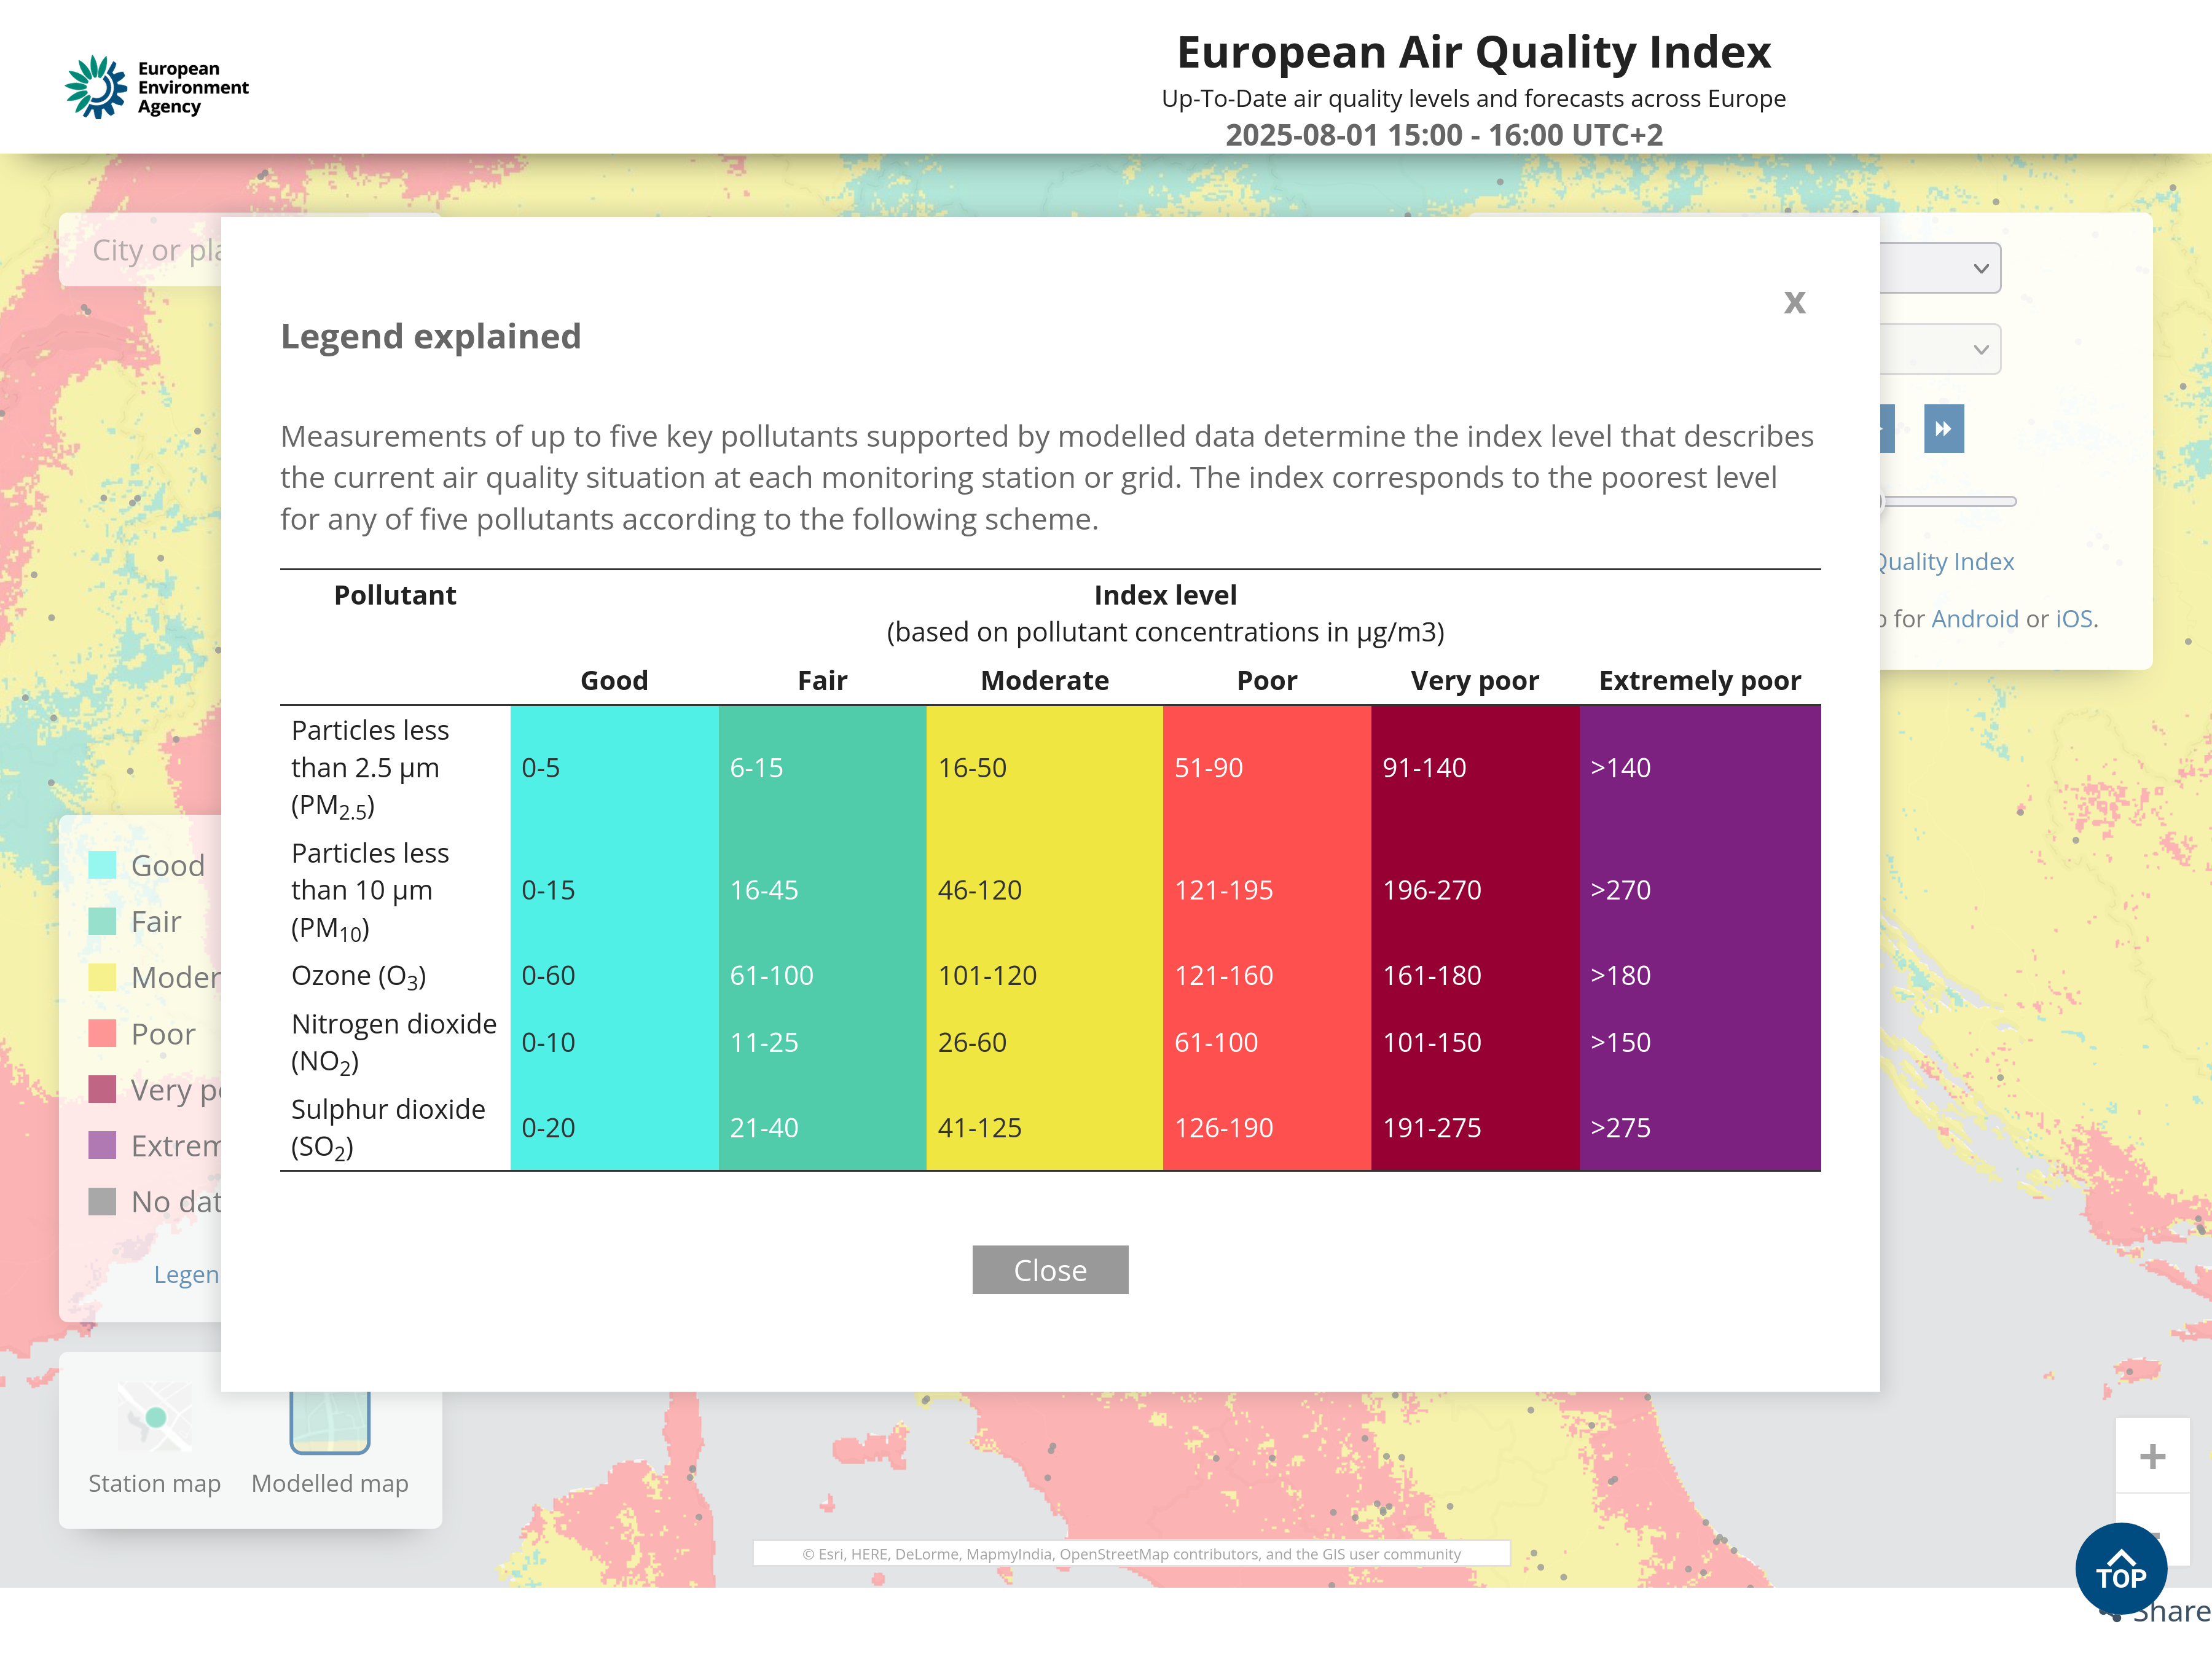
\includegraphics[width=\textwidth]{eea_4.png}
%   %\includegraphics[width=5cm]{figura.eps}%inserisce una figura larga 5cm
%   \caption[legenda elenco figure]{legenda sotto la figura}
%   \label{fig:prima}
% \end{figure}


\section{Principali inquinanti atmosferici e loro origini}

La valutazione della qualità dell'aria si basa sul monitoraggio di specifici contaminanti presenti nell'atmosfera.
Secondo \citet{GoogleMapsAirQuality2024}, i parametri più frequentemente rilevati nelle aree urbane includono:

\subsection{Materiale particolato (PM)}

Insieme di particelle microscopiche solide e liquide sospese nell'atmosfera.
Le frazioni PM$_{10}$ e PM$_{2,5}$ identificano particelle con diametro rispettivamente inferiore a 10 e 2,5 micrometri.
Le principali sorgenti comprendono:

\begin{itemize}
  \item Traffico veicolare e combustione nei motori
  \item Riscaldamento domestico a biomassa
  \item Processi industriali
  \item Fenomeni naturali come incendi boschivi e tempeste di sabbia
\end{itemize}

\subsection{Biossido di azoto NO2}

Gas caratteristico dell'inquinamento urbano, generato prevalentemente da:

\begin{itemize}
  \item Emissioni del trasporto su strada
  \item Attività industriali
  \item Impianti di produzione energetica
  \item Sistemi di riscaldamento civile
\end{itemize}

\subsection{Ozono troposferico O3}

Diversamente dall'ozono stratosferico che ci protegge dai raggi UV, quello presente negli strati bassi dell'atmosfera
costituisce un inquinante secondario. Si forma attraverso reazioni fotochimiche tra:

\begin{itemize}
  \item Composti organici volatili
  \item Ossidi di azoto
  \item Radiazione solare
\end{itemize}

Le fonti primarie dei precursori sono veicoli, centrali termoelettriche e processi industriali.

\subsection{Anidride solforosa SO2}

Gas dall'odore caratteristico e dalle proprietà irritanti, originato da:

\begin{itemize}
  \item Combustione di carbone e derivati petroliferi negli impianti energetici
  \item Raffinazione del petrolio
  \item Produzione di cemento
  \item Attività vulcanica
\end{itemize}

\subsection{Monossido di carbonio (CO)}

Gas inodore e tossico prodotto dalla combustione incompleta di combustibili fossili in veicoli e macchinari industriali.
